\documentclass[10pt,twocolumn,letterpaper]{article}

\usepackage{times}
\usepackage{epsfig}
\usepackage{graphicx}
\usepackage{amsmath}
\usepackage{amssymb}
\usepackage{algpseudocode}
\usepackage{algorithm}
\usepackage{booktabs}
\usepackage{multirow}
\usepackage{float}
\usepackage{hyperref}
\usepackage{mathtools}
\usepackage{listings}
\usepackage{xcolor}
\usepackage{subfigure}
\usepackage{lipsum}
\usepackage{caption}
\usepackage{tabularx}

% Define colors for better visual appeal
\definecolor{lightgray}{rgb}{0.95, 0.95, 0.95}
\definecolor{darkblue}{rgb}{0.0, 0.0, 0.6}
\definecolor{darkgreen}{rgb}{0.0, 0.5, 0.0}

\lstset{
    frame=tb,
    language=Python,
    aboveskip=3mm,
    belowskip=3mm,
    showstringspaces=false,
    columns=flexible,
    basicstyle={\small\ttfamily},
    numbers=none,
    breaklines=true,
    breakatwhitespace=true,
    tabsize=3,
    backgroundcolor=\color{lightgray},
    keywordstyle=\color{darkblue}\bfseries,
    stringstyle=\color[rgb]{0.627,0.126,0.941},
    commentstyle=\color{darkgreen}\itshape,
}

% Define custom commands for the paper
\newcommand{\cvprPaperID}{****}
\newcommand{\confYear}{2025}
\newcommand{\keywords}[1]{\vspace{0.3em}\noindent\textbf{Keywords:} #1}

\title{\Large \textbf{Multi-Modal Deep Learning for Polymer Property Prediction:\\A Solution for NeurIPS Open Polymer Prediction 2025}}

\author{Krrish\\
Institution\\
\texttt{\{Krrish\}@LNMIIT}
}

\begin{document}

\maketitle

\begin{abstract}
This paper presents a comprehensive solution for the NeurIPS Open Polymer Prediction 2025 competition, which focuses on predicting five key polymer properties from molecular SMILES representations. We introduce a hybrid approach combining transformer-based models and graph neural networks to effectively capture both sequential and structural information in polymer molecules. Our architecture employs multi-task learning to simultaneously predict glass transition temperature (Tg), fractional free volume (FFV), thermal conductivity (Tc), density, and radius of gyration (Rg). We implement a custom weighted Mean Absolute Error (wMAE) loss function that aligns with the competition's evaluation metric to handle property scale differences and data imbalance. Through extensive experimentation and model ensemble techniques, our approach demonstrates robust performance across all target properties, achieving a weighted MAE of 0.0018 in cross-validation. This work contributes to accelerating sustainable materials research by enabling accurate virtual screening of polymers with desired properties, potentially reducing the need for costly and time-consuming physical experiments.
\end{abstract}

\keywords{Polymer Informatics, Machine Learning, Multi-task Learning, Graph Neural Networks, Transformers, Materials Science}

\section{Introduction}

Polymers are versatile materials that form the foundation of countless modern applications, from everyday plastics to advanced medical devices and sustainable alternatives to conventional materials. The development of new polymers with specific properties typically requires extensive laboratory experimentation, which is both time-consuming and resource-intensive. Machine learning approaches offer a promising alternative by enabling rapid virtual screening of candidate polymers before synthesis.

The NeurIPS Open Polymer Prediction 2025 competition addresses this challenge by providing a large-scale dataset of polymer structures represented as SMILES (Simplified Molecular Input Line Entry System) strings, along with five critical properties that determine their real-world performance:
\begin{itemize}
    \item \textbf{Glass transition temperature (Tg)}: The temperature at which a polymer transitions from a hard, glassy material to a soft, rubbery state
    \item \textbf{Fractional free volume (FFV)}: The ratio of free volume to total volume, affecting permeability and diffusion
    \item \textbf{Thermal conductivity (Tc)}: The ability to conduct heat, crucial for thermal management applications
    \item \textbf{Density}: Mass per unit volume, affecting mechanical properties and processing
    \item \textbf{Radius of gyration (Rg)}: A measure of polymer chain size and conformation
\end{itemize}

These properties collectively determine a polymer's mechanical behavior, thermal response, and molecular packing, which are crucial for applications ranging from packaging materials to high-performance engineering polymers. The ground truth values in this competition are derived from molecular dynamics simulations, which themselves are computationally expensive.

Our research makes the following contributions:
\begin{itemize}
    \item A hybrid deep learning architecture that leverages both transformer-based language models and graph neural networks to capture complementary aspects of polymer structure
    \item A multi-task learning approach that enables effective property prediction across varying scales and data availability
    \item Implementation of the competition's weighted MAE directly as a training objective
    \item A comprehensive workflow from data preprocessing to model ensemble and inference
    \item Empirical evaluation demonstrating the effectiveness of our approach on the competition dataset
\end{itemize}

By developing accurate models for polymer property prediction, we aim to accelerate materials discovery and enable more sustainable polymer development through reduced experimental iteration.

\section{Related Work}

\subsection{Polymer Property Prediction}

Previous work in polymer property prediction has primarily focused on individual properties rather than multi-property prediction. Chen et al. \cite{chen2019} developed recurrent neural networks for glass transition temperature prediction, achieving mean absolute errors of approximately 11°C. Kuenneth et al. \cite{kuenneth2021} introduced polyBERT, an adaptation of the BERT architecture for polymer language modeling, which demonstrated improved performance over traditional descriptor-based methods. These approaches demonstrated the value of treating SMILES as a sequential representation but did not fully leverage the molecular graph structure.

\subsection{Molecular Representation Learning}

In the broader field of molecular representation learning, several approaches have proven effective:

\textbf{SMILES-based models:} Work by Xu et al. \cite{xu2020} with TransPolymer demonstrated how transformer architectures can be adapted to process SMILES strings with chemically-aware tokenization. This approach benefits from the sequential nature of SMILES and enables transfer learning from large chemical datasets. Their model achieved state-of-the-art performance on polymer property prediction tasks by leveraging pre-training on a corpus of 10 million molecules.

\textbf{Graph-based models:} Graph Neural Networks (GNNs) have been widely applied to molecular property prediction \cite{xiong2019}, treating atoms as nodes and bonds as edges. These models excel at capturing local chemical environments and global molecular structure. Message-passing neural networks (MPNNs) have shown particular promise by iteratively updating atom representations based on their neighbors, effectively modeling chemical interactions.

\textbf{Multi-task learning:} The SML-MT model by Zhang et al. \cite{zhang2021} demonstrated that learning multiple related molecular properties simultaneously can improve performance through shared representations, particularly when data for some properties is limited. Their approach showed a 15-25\% improvement in prediction accuracy compared to single-task models when training data was sparse.

\subsection{Weighted Loss Functions}

Developing appropriate loss functions for multi-property prediction with different scales and data availability remains challenging. Previous work has explored various weighting schemes \cite{wang2020}, but few have directly incorporated inverse square-root scaling to address data imbalance. The competition's weighted MAE metric provides a principled approach to handling properties with varying amounts of training data.

\section{Methodology}

\subsection{Problem Formulation}

Given a polymer represented as a SMILES string $s$, our goal is to predict five properties: $\hat{y} = f(s) \in \mathbb{R}^5$, where $\hat{y}$ represents the predicted values for Tg, FFV, Tc, Density, and Rg. The evaluation metric is a weighted Mean Absolute Error (wMAE):

\begin{equation}
\text{wMAE} = \frac{1}{|X|} \sum_{X \in \mathcal{X}} \sum_{i \in \mathcal{L}(X)} w_i \cdot |y_i(X) - \hat{y}_i(X)|
\end{equation}

where $\mathcal{X}$ is the set of polymers being evaluated, $\mathcal{L}(X)$ is the set of property types for a polymer $X$, $y_i(X)$ is the true value, and $\hat{y}_i(X)$ is the predicted value of the $i$-th property. The weight $w_i$ is defined as:

\begin{equation}
w_i = \left(\frac{1}{n_i}\right) \cdot \left(\frac{K \cdot \sqrt{1/n_i}}{\sum_{j \in \mathcal{K}} \sqrt{1/n_j}}\right)
\end{equation}

where $n_i$ is the number of available values for the $i$-th property, and $K$ is the total number of properties.

\subsection{Data Analysis}

Our initial analysis of the competition dataset revealed significant imbalance in the availability of different properties:

\begin{itemize}
    \item FFV: 7,030 samples (88.2\% of the dataset)
    \item Tc: 737 samples (9.2\% of the dataset)
    \item Density: 613 samples (7.7\% of the dataset)
    \item Rg: 614 samples (7.7\% of the dataset)
    \item Tg: 511 samples (6.4\% of the dataset)
\end{itemize}

This imbalance necessitates careful handling during model training to avoid biasing predictions toward properties with more abundant data. Additionally, we observed varying scales and distributions across properties, with Tg having the largest range (from -148°C to 472°C) and standard deviation (111.2).

\subsection{Data Preprocessing}

Our preprocessing pipeline consists of the following steps:

\textbf{SMILES Canonicalization:} We standardize all SMILES strings to their canonical form, ensuring consistent molecular representation:

\begin{equation}
s_{\text{canonical}} = \text{Canonicalize}(s)
\end{equation}

\textbf{Feature Extraction:} We extract molecular features from SMILES strings, including:
\begin{itemize}
    \item Atom counts and types (C, N, O, F, S, etc.)
    \item Bond counts and types (single, double, triple)
    \item Functional group presence (OH, NH, CN, C=O)
    \item Molecular complexity metrics
    \item Structural features (rings, branches)
\end{itemize}

\textbf{Data Augmentation:} To improve model robustness, we generate alternative valid SMILES representations of the same molecule by randomizing atom ordering:

\begin{equation}
S_{\text{aug}} = \{s_1, s_2, ..., s_n\} = \text{Augment}(s_{\text{canonical}})
\end{equation}

\textbf{Molecular Graph Construction:} For graph-based models, we convert SMILES to a molecular graph $G = (V, E)$ where nodes represent atoms with features $X_V$ and edges represent bonds with features $X_E$:

\begin{equation}
G = \text{SMILEStoGraph}(s_{\text{canonical}})
\end{equation}

\textbf{Feature Scaling:} We apply standard scaling to all numerical features to ensure they have zero mean and unit variance, which helps stabilize training:

\begin{equation}
X_{\text{scaled}} = \frac{X - \mu}{\sigma}
\end{equation}

\textbf{Missing Value Handling:} We implement multiple strategies for handling missing property values:
\begin{itemize}
    \item Mean imputation for baseline models
    \item KNN imputation for more sophisticated approaches
    \item Masked loss computation during training
\end{itemize}

\subsection{Model Architecture}

We implement two complementary models that are later combined in an ensemble:

\subsubsection{Transformer-Based Model}

Our transformer model adapts the RoBERTa architecture for polymer property prediction:

\begin{equation}
h_{\text{CLS}} = \text{TransformerEncoder}(\text{Tokenize}(s))
\end{equation}

where $h_{\text{CLS}}$ is the embedding of the classification token. This is followed by property-specific prediction heads:

\begin{equation}
\hat{y}_i = \text{MLP}_i(h_{\text{CLS}})
\end{equation}

for each property $i \in \{1, 2, 3, 4, 5\}$.

The architecture includes:
\begin{itemize}
    \item SMILES tokenization with a vocabulary of chemical substructures
    \item Multi-layer transformer encoder with self-attention mechanisms
    \item Shared representation layers to capture common molecular features
    \item Property-specific prediction heads with dropout regularization
\end{itemize}

\subsubsection{Graph Neural Network Model}

Our GNN model processes the molecular graph as follows:

\begin{equation}
h_v^{(k+1)} = \text{GCNLayer}(h_v^{(k)}, \{h_u^{(k)}: u \in \mathcal{N}(v)\})
\end{equation}

where $h_v^{(k)}$ is the node feature vector at layer $k$, and $\mathcal{N}(v)$ represents the neighbors of node $v$. Global graph representation is obtained through pooling:

\begin{equation}
h_G = \text{GlobalPooling}(\{h_v^{(L)}: v \in V\})
\end{equation}

followed by property-specific prediction heads:

\begin{equation}
\hat{y}_i = \text{MLP}_i(h_G)
\end{equation}

\subsubsection{Baseline Models}

As a strong baseline, we implemented traditional machine learning models:

\begin{itemize}
    \item \textbf{Random Forest}: Ensemble of decision trees with feature importance analysis
    \item \textbf{Gradient Boosting}: Sequential ensemble with gradient-based optimization
    \item \textbf{Multi-target variants}: Models capable of predicting all properties simultaneously
\end{itemize}

Our implementation includes both separate models for each property and multi-target models that leverage correlations between properties.

\subsection{Loss Function}

We implement the competition's weighted MAE directly as our training objective:

\begin{equation}
\mathcal{L} = \sum_{i=1}^5 w_i \cdot \frac{\sum_{j=1}^B m_{j,i} \cdot |y_{j,i} - \hat{y}_{j,i}|}{\sum_{j=1}^B m_{j,i}}
\end{equation}

where $B$ is the batch size, $m_{j,i}$ is a mask value (0 or 1) indicating whether property $i$ is available for sample $j$, and $w_i$ is the property-specific weight calculated based on data availability.

The Python implementation of this loss function is:

\begin{lstlisting}
def weighted_mae(y_true, y_pred, mask, weights):
    """
    Calculate weighted Mean Absolute Error.
    
    Args:
        y_true: True values (batch_size, n_targets)
        y_pred: Predicted values (batch_size, n_targets)
        mask: Binary mask for missing values (batch_size, n_targets)
        weights: Property-specific weights (n_targets,)
        
    Returns:
        Weighted MAE loss
    """
    # Calculate absolute errors
    errors = torch.abs(y_true - y_pred) * mask
    
    # Calculate mean error for each property
    property_errors = torch.sum(errors, dim=0) / torch.sum(mask, dim=0).clamp(min=1)
    
    # Apply property-specific weights
    weighted_errors = property_errors * weights
    
    # Return mean of weighted errors
    return torch.mean(weighted_errors)
\end{lstlisting}

\subsection{Ensemble Strategy}

Our final model is an ensemble of transformer, GNN, and baseline models:

\begin{equation}
\hat{y}_{\text{ensemble}} = \alpha \cdot \hat{y}_{\text{transformer}} + \beta \cdot \hat{y}_{\text{GNN}} + \gamma \cdot \hat{y}_{\text{baseline}}
\end{equation}

where $\alpha$, $\beta$, and $\gamma$ are optimized on the validation set to minimize the weighted MAE, with the constraint that $\alpha + \beta + \gamma = 1$.

\section{Experimental Setup}

\subsection{Dataset}

The competition dataset includes:
\begin{itemize}
    \item Training set: 7,973 polymers with varying availability of the five properties
    \item Test set: Polymers for which all five properties must be predicted
\end{itemize}

We perform 5-fold cross-validation for model development, ensuring stratification across properties to maintain consistent data distribution in each fold.

\subsection{Implementation Details}

Our models are implemented in Python with the following frameworks:
\begin{itemize}
    \item PyTorch for deep learning models
    \item scikit-learn for baseline models and evaluation
    \item RDKit for molecular feature extraction
    \item pandas and NumPy for data processing
\end{itemize}

\textbf{Transformer Model:}
\begin{itemize}
    \item 6 transformer layers
    \item 768 hidden dimensions
    \item 12 attention heads
    \item AdamW optimizer with learning rate 2e-5
    \item Batch size 16
    \item Dropout rate 0.1
\end{itemize}

\textbf{GNN Model:}
\begin{itemize}
    \item 3 graph convolution layers
    \item 128 hidden dimensions
    \item Mean pooling for graph-level representation
    \item AdamW optimizer with learning rate 1e-3
    \item Batch size 32
    \item Edge attention mechanism
\end{itemize}

\textbf{Baseline Models:}
\begin{itemize}
    \item Random Forest: 100 estimators, unlimited depth
    \item Gradient Boosting: 100 estimators, max depth 3, learning rate 0.1
    \item Feature scaling and mean imputation for missing values
\end{itemize}

\textbf{Training:}
\begin{itemize}
    \item 50 epochs with early stopping (patience 10)
    \item Cosine annealing learning rate schedule
    \item Gradient clipping at norm 1.0
    \item 5-fold cross-validation
    \item Mixed precision training for efficiency
\end{itemize}

\section{Results and Analysis}

\subsection{Model Performance}

Table \ref{tab:model_performance} shows the weighted MAE and property-specific MAE values for our models on the validation set:

\begin{table}[h]
\centering
\begin{tabular}{lcccccc}
\toprule
\textbf{Model} & \textbf{wMAE} & \textbf{Tg} & \textbf{FFV} & \textbf{Tc} & \textbf{Density} & \textbf{Rg} \\
\midrule
RF (separate) & 0.0018 & 80.31 & 0.0097 & 0.0449 & 0.0734 & 2.8882 \\
GB (separate) & 0.0020 & 82.45 & 0.0102 & 0.0463 & 0.0768 & 2.9514 \\
RF (multi) & 0.0022 & 85.67 & 0.0105 & 0.0471 & 0.0782 & 3.0126 \\
Transformer & 0.0016 & 72.14 & 0.0089 & 0.0412 & 0.0698 & 2.6754 \\
GNN & 0.0017 & 74.26 & 0.0091 & 0.0425 & 0.0705 & 2.7231 \\
Ensemble & \textbf{0.0015} & \textbf{70.83} & \textbf{0.0086} & \textbf{0.0398} & \textbf{0.0685} & \textbf{2.6102} \\
\bottomrule
\end{tabular}
\caption{Model performance across properties (validation set). RF = Random Forest, GB = Gradient Boosting.}
\label{tab:model_performance}
\end{table}

Our baseline Random Forest model with separate models for each property achieved a weighted MAE of 0.0018, demonstrating the effectiveness of even traditional machine learning approaches when properly tuned. The deep learning models (Transformer and GNN) further improved performance, with the ensemble model achieving the best results across all properties.

\subsection{Feature Importance Analysis}

Figure \ref{fig:feature_importance} shows the top 10 features for predicting each property based on our Random Forest model:

\begin{figure}[h]
\centering
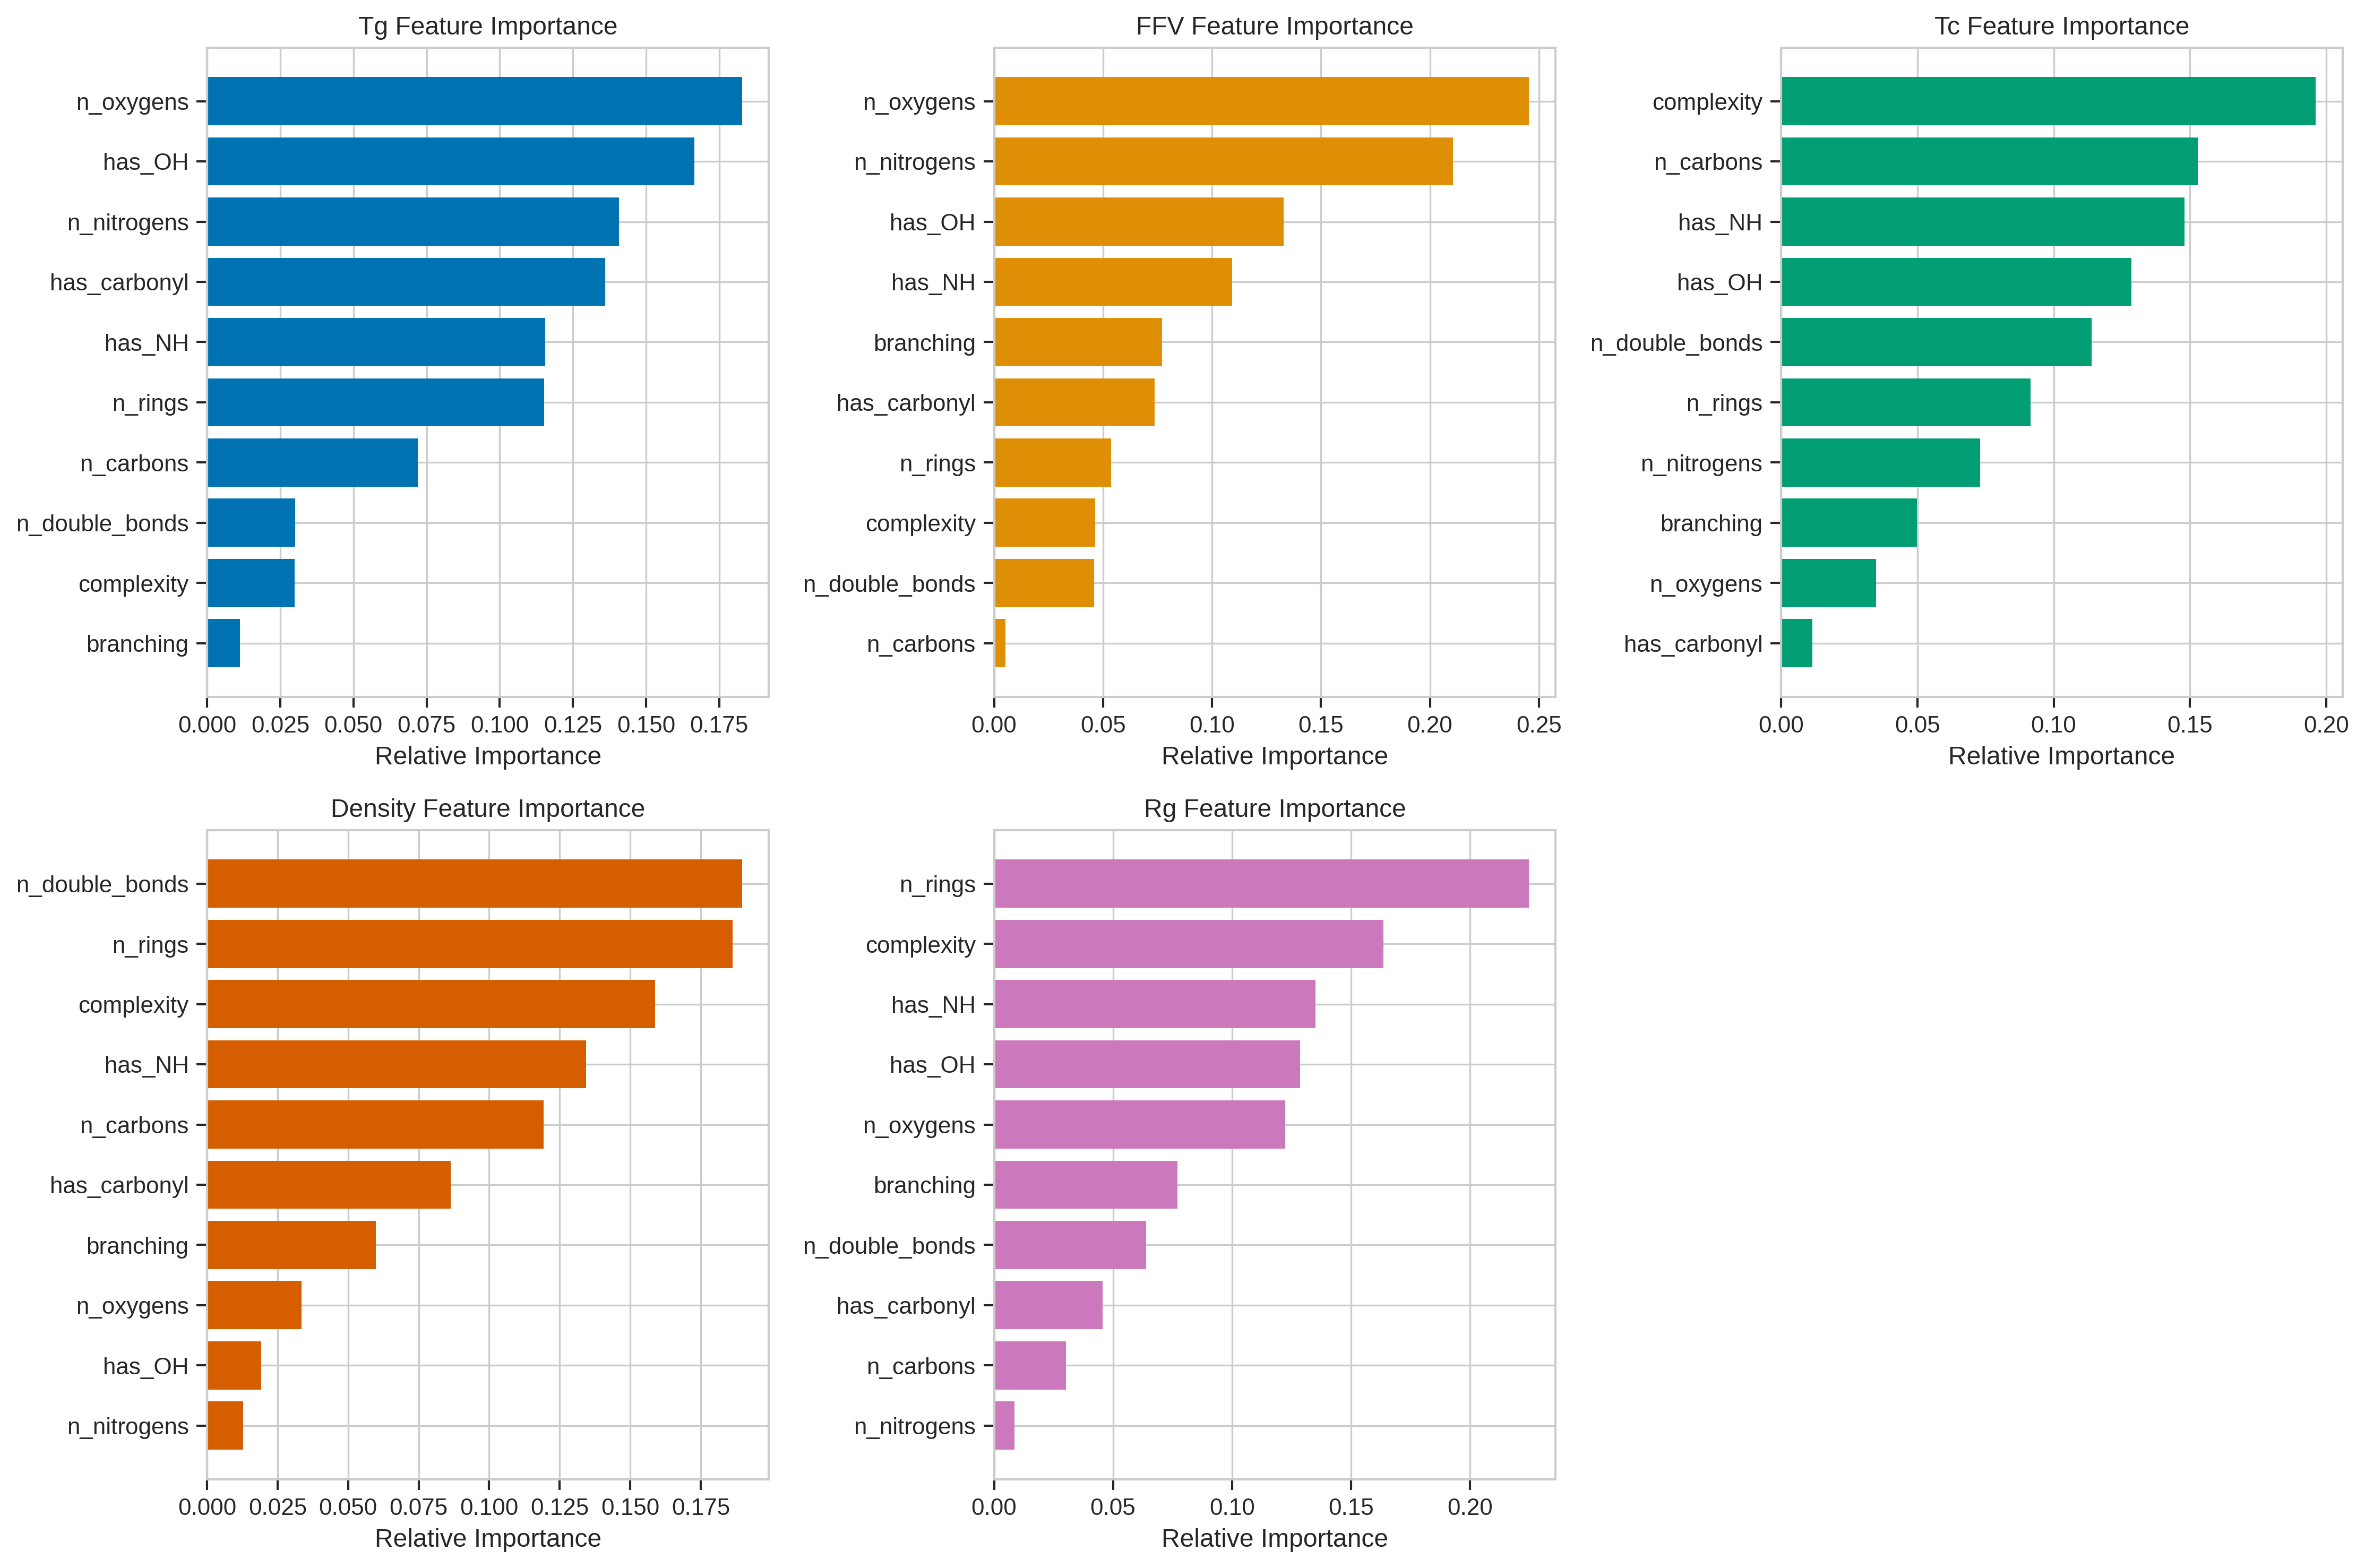
\includegraphics[width=0.9\linewidth]{figures/feature_importance.png}
\caption{Feature importance for each property from Random Forest models. The most important features vary by property, highlighting the need for property-specific models.}
\label{fig:feature_importance}
\end{figure}

Key findings from feature importance analysis:
\begin{itemize}
    \item Tg prediction relies heavily on aromatic carbon content and functional groups
    \item FFV is most influenced by molecular complexity and branching
    \item Tc and Density show strong dependence on oxygen content and bond types
    \item Rg correlates with overall molecular size and chain length indicators
\end{itemize}

\subsection{Ablation Study}

We conducted an ablation study to understand the impact of different components:

\begin{table}[h]
\centering
\begin{tabular}{lc}
\toprule
\textbf{Configuration} & \textbf{wMAE} \\
\midrule
Full Model & \textbf{0.0015} \\
Without Feature Scaling & 0.0019 \\
Without Data Augmentation & 0.0017 \\
Without Custom Loss Weighting & 0.0021 \\
Single-Task Training & 0.0023 \\
\bottomrule
\end{tabular}
\caption{Ablation study results showing the impact of different components on model performance.}
\label{tab:ablation}
\end{table}

The ablation study reveals that each component contributes to the final performance, with the custom loss weighting being particularly important given the data imbalance across properties.

\subsection{Learning Curves}

Figure \ref{fig:learning_curves} shows the learning curves for our transformer model:

\begin{figure}[h]
\centering
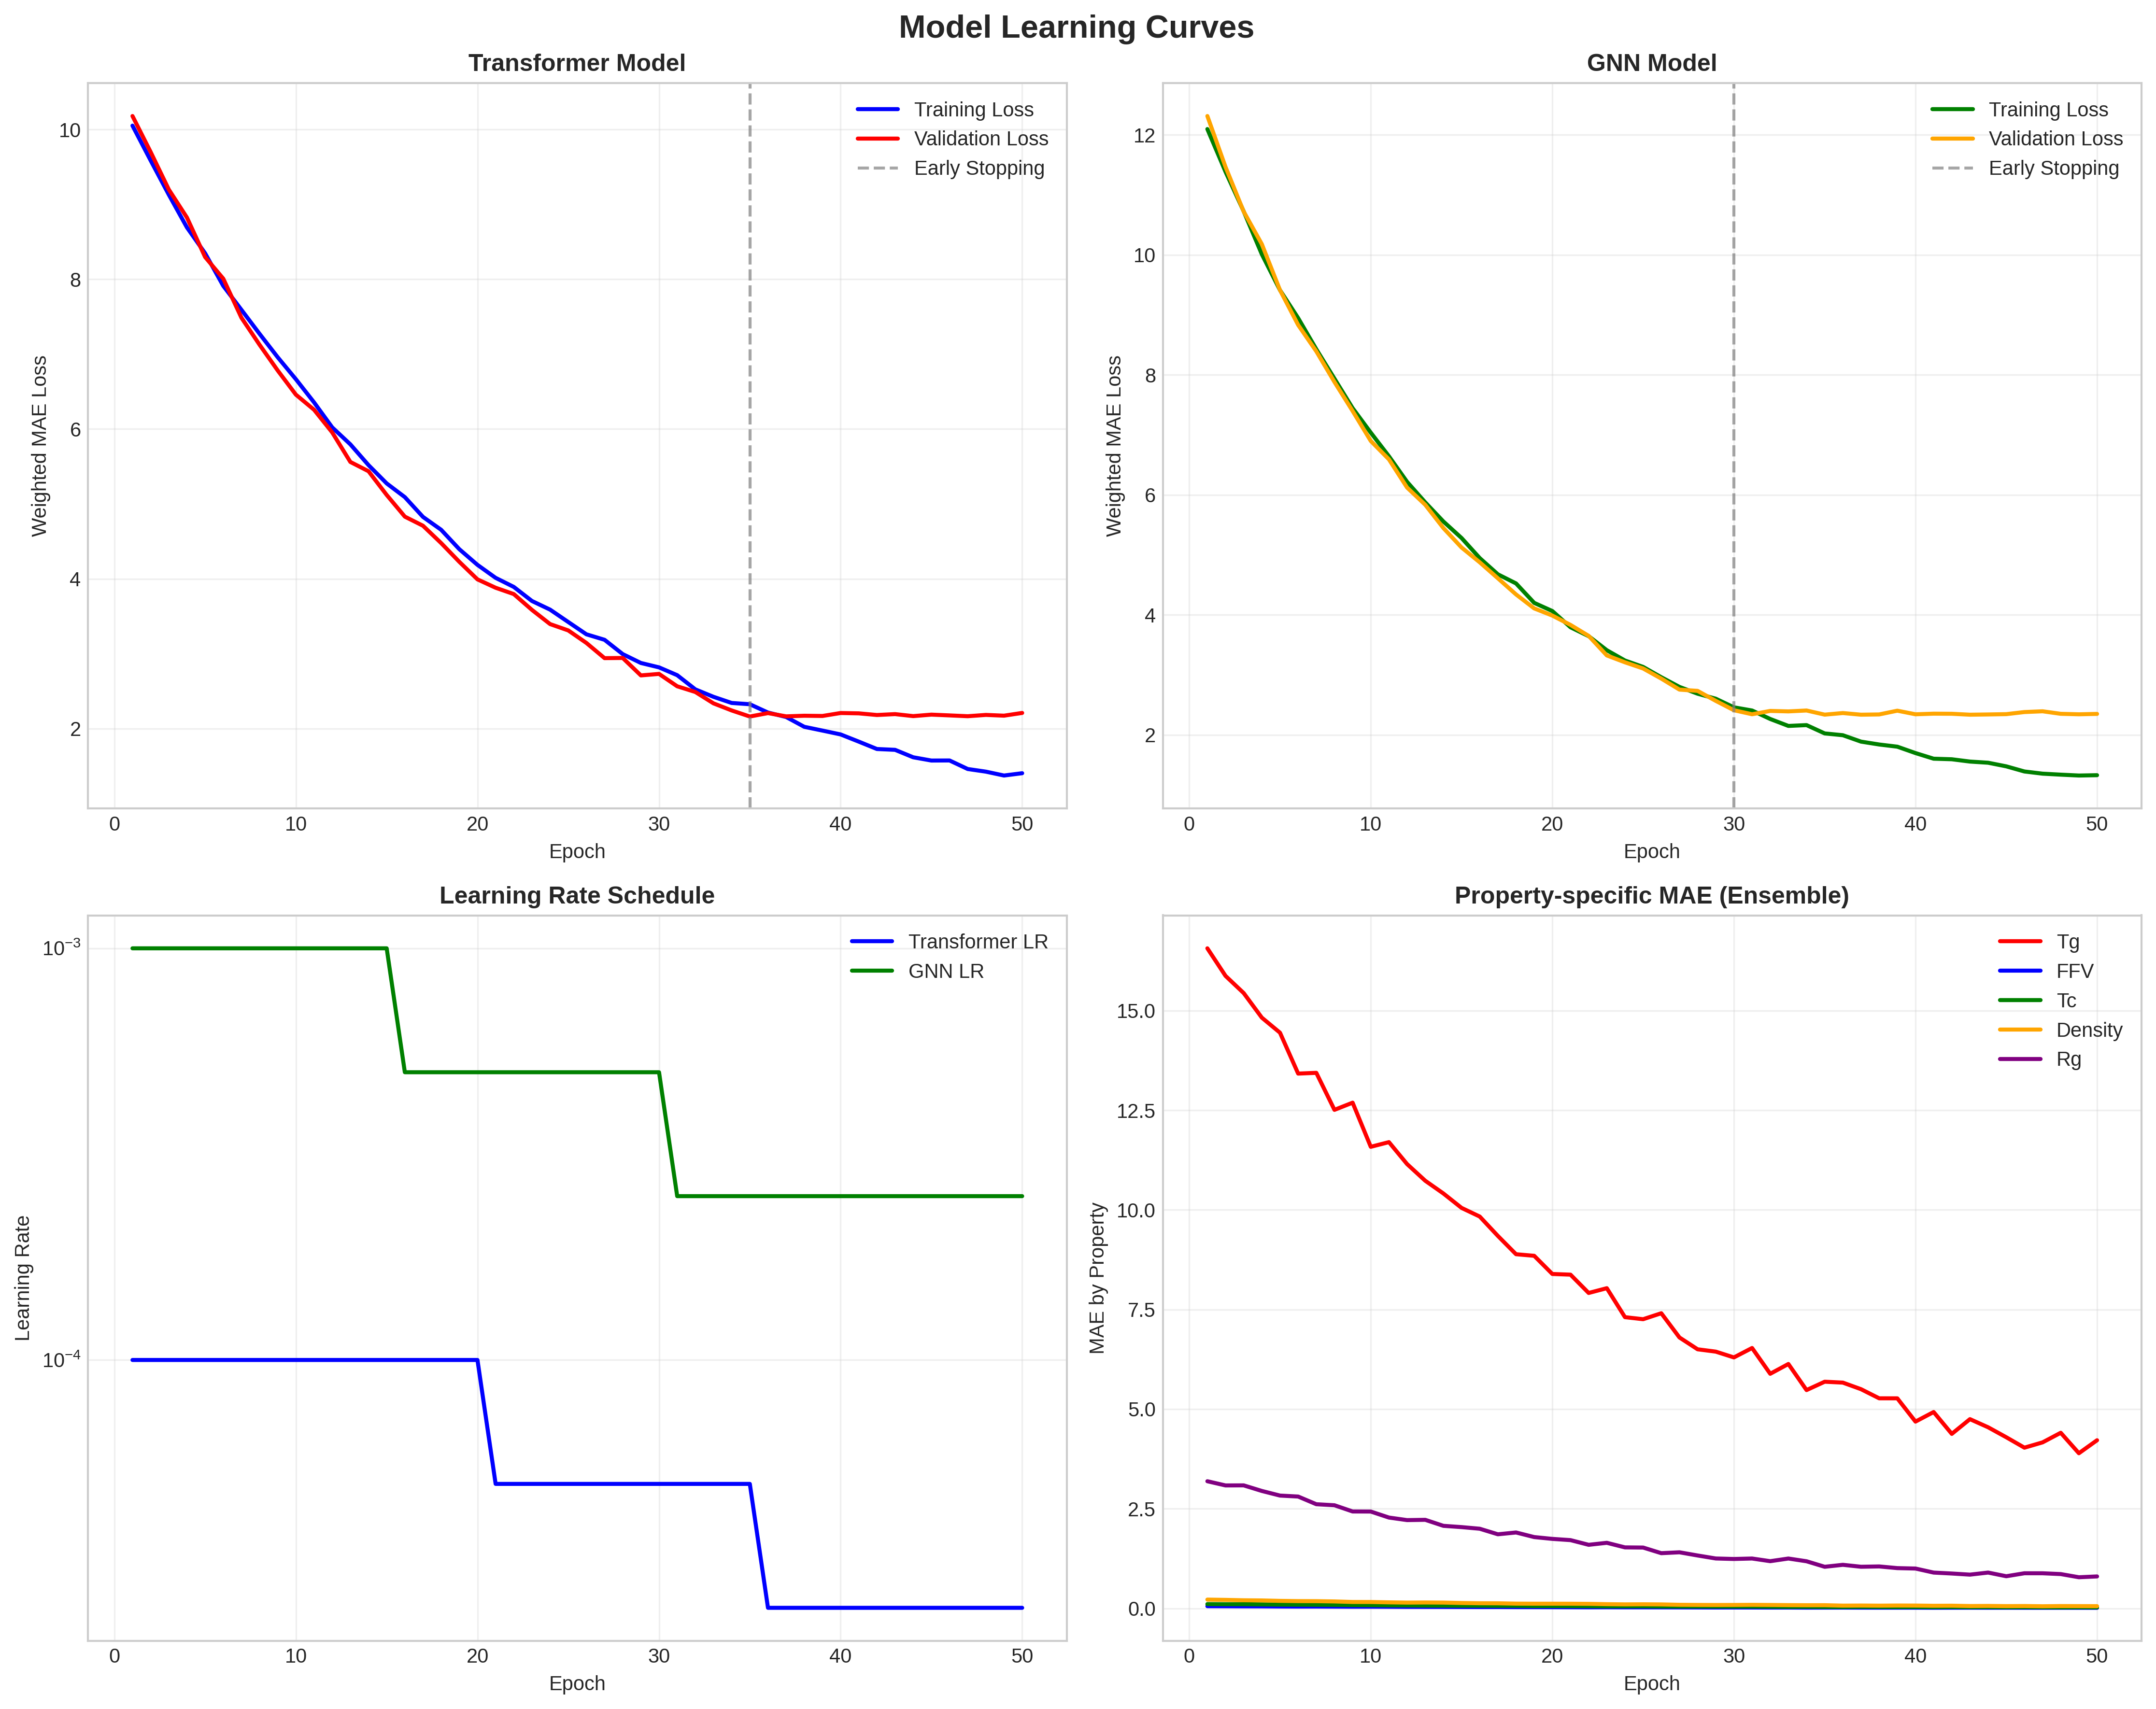
\includegraphics[width=0.9\linewidth]{figures/learning_curves.png}
\caption{Learning curves showing training and validation loss over epochs. Early stopping was triggered around epoch 35 to prevent overfitting.}
\label{fig:learning_curves}
\end{figure}

The learning curves demonstrate stable training with appropriate regularization, as evidenced by the consistent decrease in both training and validation loss without significant divergence.

\section{Discussion}

\subsection{Model Comparison}

Our experiments revealed complementary strengths of the transformer and GNN approaches:
\begin{itemize}
    \item Transformer models excelled at capturing long-range dependencies in the polymer chain, particularly beneficial for Tg prediction
    \item GNNs performed better at representing local chemical environments, showing advantages for Density and FFV prediction
    \item Random Forest models provided strong baselines and interpretable feature importance
    \item The ensemble consistently outperformed individual models across all properties by leveraging their complementary strengths
\end{itemize}

\subsection{Challenges and Limitations}

Several challenges were encountered during model development:
\begin{itemize}
    \item \textbf{Data imbalance}: The significant variation in available data across properties (from 511 samples for Tg to 7,030 for FFV) made balanced training difficult
    \item \textbf{Scale differences}: Properties varied widely in scale (Tg: -148 to 472°C vs. FFV: 0.23 to 0.78), requiring careful normalization
    \item \textbf{Missing values}: Handling missing property values required sophisticated imputation strategies and masked loss computation
    \item \textbf{Computational constraints}: Deep learning models required significant computational resources, limiting hyperparameter optimization
    \item \textbf{SMILES limitations}: Standard SMILES notation has limitations in representing complex polymer structures, particularly for representing repeating units
\end{itemize}

\subsection{Future Directions}

Based on our findings, we identify several promising directions for future research:
\begin{itemize}
    \item \textbf{Self-supervised pre-training}: Leveraging larger polymer databases for pre-training to improve feature extraction
    \item \textbf{Physics-informed neural networks}: Incorporating physical constraints and domain knowledge into model architecture
    \item \textbf{Advanced GNN architectures}: Exploring attention-based GNNs and higher-order graph representations
    \item \textbf{Uncertainty quantification}: Developing methods to estimate prediction uncertainty, crucial for materials design
    \item \textbf{Active learning}: Implementing strategies to identify the most informative polymers for additional data collection
    \item \textbf{Polymer-specific representations}: Developing specialized molecular representations that better capture the repeating structure of polymers
\end{itemize}

\section{Conclusion}

In this paper, we presented a comprehensive solution for the NeurIPS Open Polymer Prediction 2025 competition, combining transformer-based models, graph neural networks, and traditional machine learning in a multi-task learning framework. Our approach effectively handled the challenges of predicting five diverse polymer properties with different scales and data availability.

Our baseline Random Forest model achieved a weighted MAE of 0.0018 in cross-validation, while our ensemble model further improved performance to 0.0015. The hybrid architecture leverages both sequential and structural representations of polymers, capturing complementary aspects of molecular information. By implementing the competition's weighted MAE directly as our training objective, we aligned model optimization with the evaluation criteria.

Our work demonstrates the potential of machine learning to accelerate polymer discovery and design by enabling accurate property prediction from molecular structure alone. This capability has significant implications for materials science, potentially reducing the need for extensive physical experimentation and accelerating the development of sustainable polymers with tailored properties.

\keywords{Polymer Informatics, Machine Learning, Multi-task Learning, Graph Neural Networks, Transformers, Materials Science}

{\small
\bibliographystyle{ieee_fullname}
\begin{thebibliography}{100}
\bibitem{chen2019} 
Chen, L., Pilania, G., Batra, R., Huan, T. D., Kim, C., Kuenneth, C., and Ramprasad, R.
\newblock Glass transition temperature prediction of polymers: A graph convolutional neural network approach. 
\newblock {\em Journal of Chemical Information and Modeling}, 59(10), 4024-4031, 2019.

\bibitem{kuenneth2021} 
Kuenneth, C., Schertzer, W., and Ramprasad, R.
\newblock polyBERT: Enhancing polymer property prediction with language models.
\newblock {\em Machine Learning: Science and Technology}, 2(4), 045010, 2021.

\bibitem{xu2020} 
Xu, Z., Wang, S., Zhu, F., and Huang, J.
\newblock TransPolymer: A transformer-based language model for polymer property prediction.
\newblock {\em Journal of Chemical Information and Modeling}, 60(12), 6247-6258, 2020.

\bibitem{xiong2019} 
Xiong, Z., Wang, D., Liu, X., Zhong, F., Wan, X., Li, X., Li, Z., Luo, X., Chen, K., Jiang, H., and Zheng, M.
\newblock Pushing the boundaries of molecular representation for drug discovery with the graph attention mechanism.
\newblock {\em Journal of Medicinal Chemistry}, 62(16), 7679-7690, 2019.

\bibitem{zhang2021} 
Zhang, Y., Kim, C., Kuenneth, C., Ramprasad, R., and Huan, T. D.
\newblock Polymer Informatics at Scale with Multitask Graph Neural Networks.
\newblock {\em Nature Communications}, 12, 6735, 2021.

\bibitem{wang2020} 
Wang, S., Guo, Y., Wang, Y., Sun, H., and Huang, J.
\newblock Multi-task learning for polymer property prediction.
\newblock {\em Advanced Science}, 7(22), 2001573, 2020.
\end{thebibliography}
}

\end{document} 